\subsubsection{Goals}

TLEP, Triple Large Electron Positron, is an $e^+ e^-$ circular collider of circumference 80km. It will probe the properties of the Higgs H(126) boson with unmatched accuracy thanks to greater luminosity compared to other designs \cite{TLEP:Review}. In an effort to complete the Standard Model of particle physics, TLEP will also investigate the properties of the Z and W bosons and the top quark. 

Mapping the electroweak symmetry-breaking parameters will lead to stringent Standard Model closure tests. TLEP expects to be able to take direct measurements of the mass of W and top quark with an order of magnitude improvement and improve on the mass of Z pole by two orders of magnitude. \cite{TLEP:Janot}

\subsubsection{Technical Specification}

\begin{figure}[!htb]
  \centering
  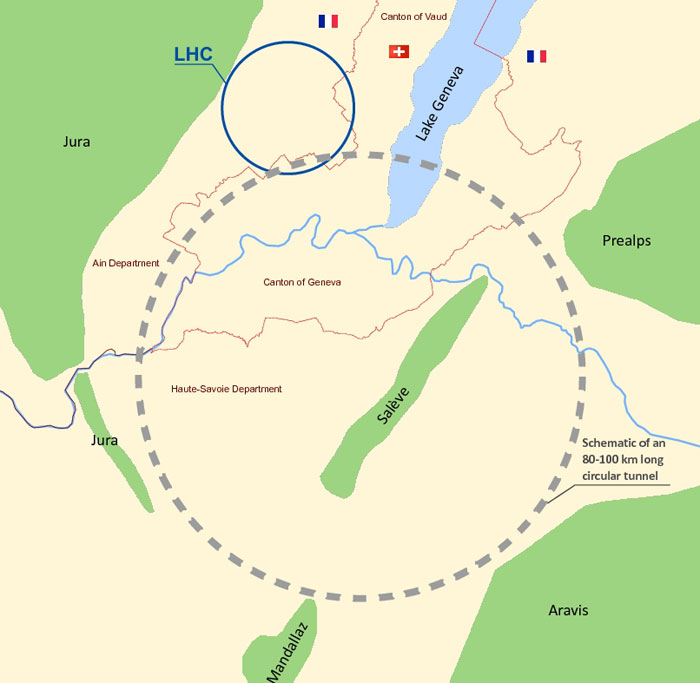
\includegraphics[width=0.6\textwidth,natwidth=700,natheight=683]{TLEP_Diagram.jpg}
  \caption{Proposed TLEP site next to LHC}
\end{figure}

TLEP's primary potential site is an 80km ring at CERN encompassing the LHC along part of the circumference. The design began as LEP3, a proposed improvement to the LHC which has been put aside in favour of TLEP due to its superior parameters, the fact it can be implemented without halting the operation of the LHC and the upgrade potential \cite{TLEP:Luminosity}. Table \ref{TLEP:Specs} shows a summary of the luminosities achievable with TLEP alongside LEP3 design for comparison. Luminosity figures for TLEP are upwards of one order of magnitude greater than any other proposed design.

\begin{table}
\centering
\begin{tabular}{l|cc}
  & LEP3 & TLEP \\
  \hline
  Circumference & 26.7km & 80km \\
  Max. Beam Energy (GeV) & 120 & 175 \\
  Luminosity @ 350 GeV ($cm^{-2} s^{-1}$) & \textendash & $0.7 \times 10^{34}$ \\
  Luminosity @ 240 GeV ($cm^{-2} s^{-1}$) & $10^{34}$ & $5 \times 10^{34}$ \\
  Luminosity @ 160 GeV ($cm^{-2} s^{-1}$) & $ 5 \times 10^{34}$ & $2 \times 10^{35}$ \\
  Luminosity @ 90 GeV  ($cm^{-2} s^{-1}$) & $2 \times 10^{35}$ & $10^{36}$ \\
\end{tabular}
  \caption{Parameters for performance of LEP3 and TLEP \cite{TLEP:AccNews}}
  \label{TLEP:Specs}
\end{table}

The main operational mode of TLEP will be at 240 GeV in order to function as a Higgs factory, however TLEP will be operating between 90 GeV, to probe the Z pole interactions, through 160 GeV to investigate W bosons, up to 350 GeV to investigate the properties of the top and anti-top quarks ($t\bar{t}$). The substantially higher luminosity compared to other designs comes from the 4 interaction points possible with the circular design, resulting in a greater number of observable interaction events per year. These specifications will result in the observation of roughly 2 million Higgs decays over a five year exposure \cite{TLEP:CERNReport}. Unparalleled beam energy accuracy is achieved by the method of transverse polarisations of the beams \cite{TLEP:Review}.

\subsubsection{Technical Feasibility}

The main focus of R\&D and cost driver will be the power requirements of the RF system. Currently CERN has a contract with France's main energy supplier EDF for 200 MW \cite{TLEP:Luminosity}. Early estimates on the power requirements of TLEP running at 175 GeV beam energy will be in the region of 280 MW, using scaled\textendash up values from the LHC and other projects. Synchrotron radiation is the main source of power loss dnd this is the main area for R\&D. The current design study benchmark is 54-59\% efficiency of the RF system \cite{TLEP:Review}. At present the extraction of 100 MW of power in the form of heated water is a design consideration that has yet to be addressed.

% todo beamstrahling?
The interference of beam-beam interactions resulting in loss of power of the beam and in turn lower luminosity is known as bremsstrahlung and must be mitigated in a successful circular collider even though the effect is far less than for linear models \cite{TLEP:Luminosity}. Estimates of acceptable momentum are in the region of 2-2.5\%. Simulations show that with a momentum acceptance of 2.5\% a beam lifetime of 460$\pm$50 s is achievable \cite{TLEP:EnergyRestriction}. Another option is to increase the ratio of horizontal to vertical emittance – producing flattened beams. LEP showed that an emittance ratio of 250 is achievable, however R\&D is needed to bring this figure closer to that of modern light sources of O(2000).

For an upper limit of the beam lifetime due to Bhabha scattering of O(1000s) 1\% of the total beam energy needs to be reintroduced every 10s \cite{TLEP:Janot} \cite{TLEP:CERNOverview}. This requires an injector and separate accelerator ring working alongside the primary ring that must be designed and considered for injector strength, power consumption and the shielding required to block the accelerator ring from the detectors. 

Detector systems are yet to be designed but those of the LHC, PEP II and KEKB experiments, among others, can be used as benchmarks. The unprecedented quantity of data available from such high luminosities requires evaluation of computing needs against currently used systems. 

\subsubsection{Cost and Schedule}

It is expected that the initial design study, reporting fully on the above main technical points, will be completed by 2015. This will be followed by an in depth conceptual and R\&D study phase with technical design of critical components to be completed by 2017-18 \cite{TLEP:CERNOverview}. These findings can then be presented at the next European Strategy update after which an informed decision on the next high-energy frontier project can be carried out and properly implemented. Construction could begin by 2020 with completion and operation by 2030. 

TLEP's preliminary cost estimates have been based largely on the fact that the design utilises fairly mature technologies and many of the contributions to cost estimates have been arrived at by scaling up existing projects. However with the technical challenges still to overcome it is impossible to arrive at anything but very rough estimates of an overall budget. Current estimates place the total cost at 7 billion Swiss Francs, of the same order as the LHC and ILC design \cite{TLEP:Janot}. Of this value half is projected to be the digging of the tunnel itself and it is important to note detector cost has not been factored into this value.

\subsubsection{Potential}

TLEP has a highly promising potential upgrade path. Following the fulfilment of the experimental objectives within a reasonable lifespan of the project ($\sim$40 years from present), TLEP can undergo combination with the LHC to form the VHE-LHC, a 100 TeV proton-proton collider with the LHC serving as an injector ring \cite{TLEP:Janot}. This provides a robust long-term vision for high energy physics and the CERN facilities with the promise of precision measurements and potential for discovery at an energy frontier higher than any alternative. The return of investment on each facility by repurposing them together financially trumps the costs of all other long-term design schemes as they stand at present.
